\chapter{Bound diffusion measurements}\label{ch04}
\label{ch:bound-diffusion}

Following up on the principles of the bound-diffusion theory, we wanted to see whether we could measure bound diffusion in a biomaterial inspired by the nuclear pore complex.  In order to do that, we made Nup-filled hydrogels and measured the diffusion of transport factors and inert proteins within them.  We measured the diffusion in a few different ways: monitoring the concentration profile and total accumulation as the proteins diffused into the cell, and using fluorescence recovery after photobleaching (FRAP).
\section{Experimental setup}
\subsection{Hydrogels}
Applying the lessons learned in the previous chapter, the nuclear pore mimics were 6\% acrylamide hydrogels with FSFG-bis anchored in.  The precursor solution had a final concentration of 6\% premixed acrylamide/bisacrylamide (29:1) in PTB pH 7.0.  The crosslinker was either 1 mM LAP or 0.1\% ammonium persulfate and 0.5\% TEMED (check these concentrations).  Lyophilized FSFG-bis was resuspended in PTB, allowed to sit at room temperature for at least 20 minutes, and added to the precursor solution.  I used nominal FSFG concentrations between 5 and 10 mg/mL, depending on whether it was FSFG concat 1 or FSFG concat 2.  If a photoinitiator was used, it was added in the darkroom, and the solution was protected from light as much as possible afterwards.

After the precursor solution was thoroughly mixed, it was degassed in a vacuum desiccator for 10 minutes and immediately pipetted into a disassembled 400-$\mu$m-thick PDMS gasket chamber. Drops between 0.5 and 2 $\mu$L were carefully pipetted onto the plastic slide and the chamber assembled around the drops.  Typically, each chamber measured a few centimeters on a side and contained a control gel with no Nups as well as one or more Nup-filled gels.  The chamber was then illuminated with UV light at some intensity that I will look up as uniformly as possible for 30 seconds using a ThorLabs etc. LED.  Condensation around the gels indicated that they had crosslinked.  The chamber was immediately rinsed with at least 100 $\mu$L of PTB, filled with fresh PTB, and sealed with PDMS and clingwrap.  The gels were left to soak at 4$^\circ$C for at least 12 hours so that any remaining precursor solution and protein could leave the gel.

\subsection{Binding affinity of NTF2 and FSFG}
% ITC data is in book 1, a bit of book 2.  None of the fits were good.  Data shown here is taken from the runs on 6/18/14 and 6/23/14.  Fits aren't shown because we never really understood them.
Although bound diffusion is the key parameter from our reaction-diffusion model of selectivity, the kinetic parameters of off-rate $\koff$, on rate $\kon$, and dissociation constant $K_D = \koff/\kon$ are also important. These parameters are surprisingly difficult to measure, yielding values between 10 nM and 10 $\mu$M depending on the experimental conditions.  We estimated the dissociation constant for NTF2 and FSFG concat-1 using isothermal titration calorimetry (ITC).  The heat of injection was recorded as FSFG was titrated into a stock of NTF2.  While the resulting titration curves had low signal-to-noise and did not reach saturation, they clearly indicated binding (Fig.~\ref{fig:ITC-runs}).  Simple fits are likely inaccurate, given the high degree of multivalent binding, but may provide an order-of-magnitude estimate of the affinity.  Several ITC curves agree on a dissociation constant of $K_D \approx 200 \mu$M.  This is roughly compatible with the millimolar per-FSFG constant measured by the Rout lab with NMR and ITC \cite{hayama18}.  Similarly weak values were predicted through NMR, simulation, and stopped-flow anisotropy \cite{milles15}.

\begin{SCfigure}
\caption{Isothermal calorimetry titration curve: heat of injection vs. molar ratio of FSFG to NTF2. Fits are questionable but multiple runs suggest $K_D \approx 200\ \mu$M.\\}
\centering
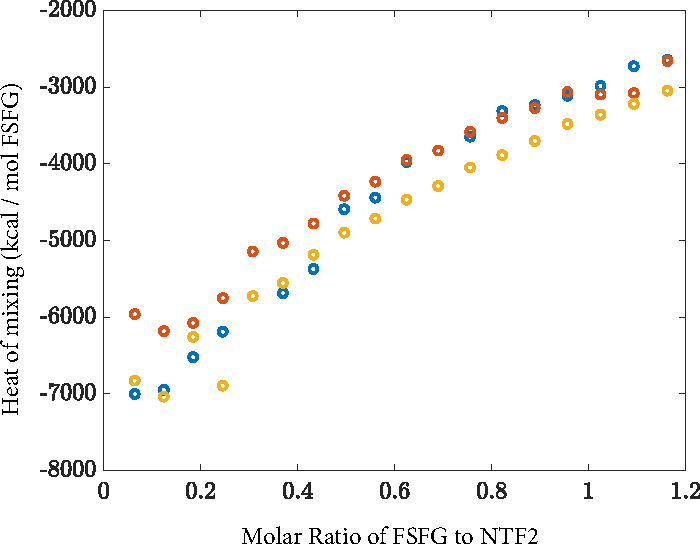
\includegraphics[width=0.6\textwidth]{figs/ch04/ITC_runs}
\label{fig:ITC-runs}
\end{SCfigure} 

Due to the twin difficulties of varying $K_D$ in a controlled way and accurately measuring its value, we did not attempt to experimentally alter this parameter.  Ideally, a transport factor - Nup pair with $K_D \approx 1 \mu$M would have been used to maximize selectivity.  For the purposes of determining the bound diffusion constant, the only value that is necessary to measure is the ratio $K_D/N_T$, which can be estimated using the partitioning of transport factors and inert proteins into the FSFG hydrogels (Sec.~\ref{sec:part-coeff}).  We investigated using the ubiquitin-associated (UBA) domain of the mRNA exporter Mex67 as a Nup-binding domain in GFP fusion proteins.  In principle, varying numbers of this small ($<$10 kDa) domain could be added to GFP to explore the effect of varying binding affinity and valency in transport factors.  The constructs GFP-UBA, GFP-UBAx2, and GFP-UBAx3 were created by Eric Verbeke, but did not express and/or bind well.

%Eric did most of the UBA cloning I think
% Expression tests in LKM book 5 pgs 146-9

\subsection{Quantifying concentration of Nups in the hydrogels}

The remaining potentially-tunable parameter of the bound-diffusion model is $N_T$, the total concentration of tethered Nups.  It is straightforward to control the Nup concentration in the hydrogel precursor solution by resuspending a known mass of lyophilized proteion.  Nup concentrations up to $\sim 50$ mg/mL can be resuspended.  However, it is much more difficult to determine how much protein was tethered to the hydrogel upon crosslinking. 

 BCA protein quantitation assays were used to place upper bounds on $N_T$.  Two methods were attempted: incubating the hydrogel itself in the working reagent, and soaking the hydrogel in a known volume of buffer and testing the concentration of FSFG released.  When applying the first method, the hydrogel was first soaked to remove excess precursor solution and thoroughly rinsed.  The gel was placed into a 96-well plate and buffer added until the appropriate sample volume was reached.  A standard BCA protocol was then followed.  Upon incubation with the working reagent, the hydrogels turned purple, as expected.  Standard absorption measurements and processing yielded an estimate of 0.5 mg/mL tethered FSFG-concat 1; this should be taken as an approximate value only.  The second method, that of soaking hydrogels and measuring the FSFG released, placed a similarly-low upper bound on tethered FSFG concentration.  Hydrogels made with 5 $\mu$L of precursor solution were soaked in 45 $\mu$L buffer to equilibrate.  The buffer was then measured to have a concentration of 1.0 mg/mL FSFG, implying a tethered FSFG concentration of $<1$ mg/mL.
% LKM book 5 pgs 119 and later

The concentration of Nups within the pore may reach 100 mg/mL \cite{thing}.  The low concentration of tethered Nups that we were able to achieve is therefore a major barrier to selectivity.  It is likely that the disordered nature of FSFG makes the labeled end less accessible to the hydrogel scaffold than would be the case for an ordered protein.  In an effort to overcome this limitation, we tested other linkers and conjugation methods.  We conjugated the FSFG-cys to PEG-diacrylate of varying lengths (700 Da and 10 kDa), to multi-armed PEG-diacrylate, and to maleimide-PEG-acrylate.  While labeling was verified using Ellman's reagent (Appendix~\ref{appx:bis-labeling}), there was no noticeable difference in transport factor partitioning into these hydrogels.
% maleimide-PEGDA LKM book 6 pgs 7-10
% multi-armed PEGDA LKM book 5 pg 151
% basic PEGDA conjugations throughout book 5

\subsection{Influx experiments}
After soaking in buffer, the buffer solution was removed by pipette or wicking with a Kimwipe (not by aspirating) and a fluorescent reservoir solution added.  The reservoir solution contained 20 $\mu$M each NTF2-fluorescein (NTF2-F) and mCherry in PTB.  The chamber was resealed after adding the solution.  If a profile and accumulation experiment was being run, the experiment was run immediately after adding the reservoir solution.  Experiments were run on an Olympus widefield using a 4x objective with FITC and TRITC filter cubes (should I put exact specifications here).  Typical experiments were run for 120 minutes at a rate of one frame per minute.  Exposure times were usually 30-100 ms with 3-8 dB gain in both channels.  Minimal photobleaching took place over the course of these experiments.  Data was analyzed as described below.  After the end of an influx experiment, the chamber could be stored at 4$^\circ$C, protected from light, for a further 12-24 hours in order to equilibrate.  A FRAP experiment could then be performed.

 % '/Volumes/houghgrp/Processed Images/2019-2-21_5/results.mat'
%'/Volumes/houghgrp/Microscopy/190220/190220_profiles_02.vsi’
%Cct2
%grnScale = [0;0.07];
%redScale = [0.0183566033417258;0.0502479591058213];
%Image_series_figures.m
\begin{figure}
\caption{Influx image series}
\centering
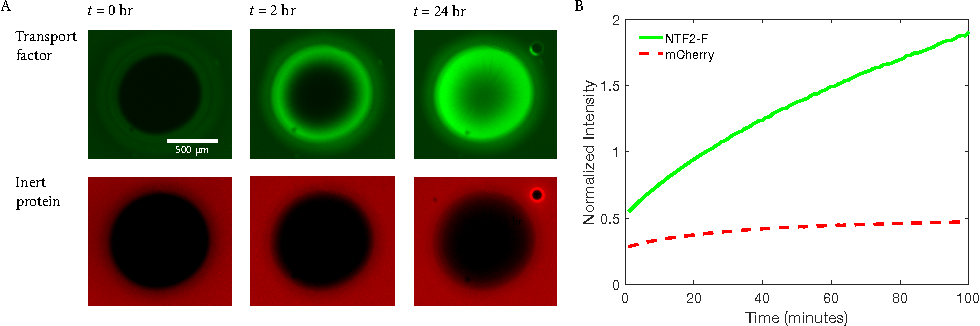
\includegraphics[width=\textwidth]{figs/ch04/influx-images-clean.pdf}
\label{fig:influx-images}
\end{figure} 

\begin{SCfigure}
\caption{Influx plot series \\}
\centering
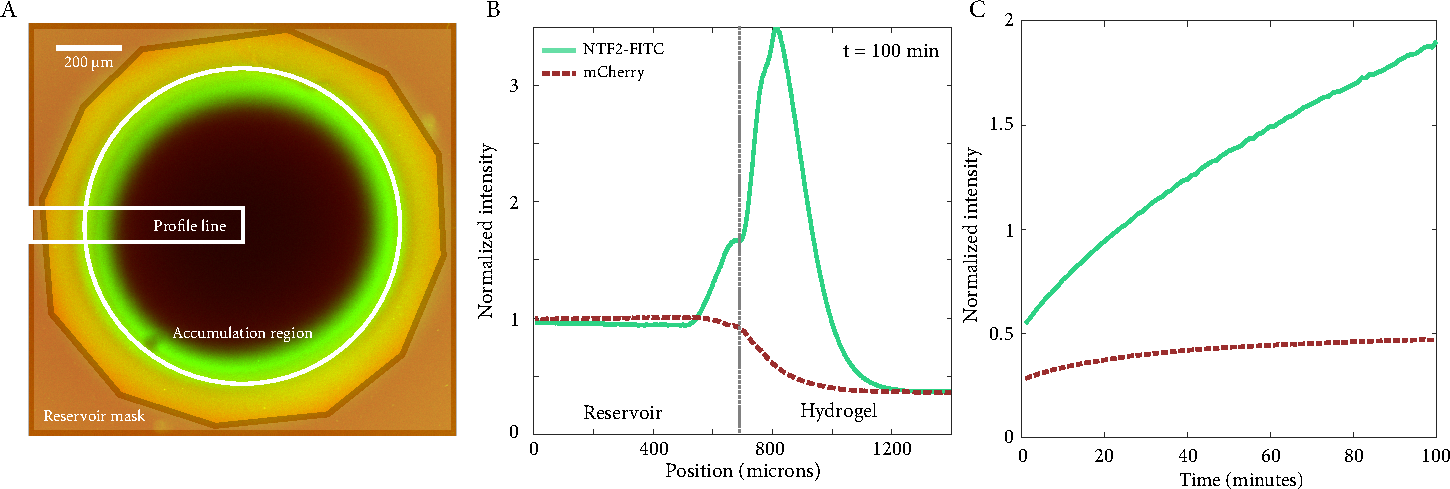
\includegraphics[width=0.7\textwidth]{figs/ch04/influx-plots.pdf}
\label{fig:influx-plots}
\end{SCfigure} 

\subsection{Fluorescence recovery after photobleaching}
Fluorescence recovery after photobleaching (FRAP) relies on the redistribution of fluorophores after patterned photobleaching in order to determine their diffusion constant.  After a small portion of the hydrogel is bleached, the bleached spot gradually exchanges with the non-bleached fluorophores outside, and the average fluorescence intensity within the bleached spot recovers.  The recovery lifetime can be used to determine the fluorophore's diffusion constant, and the final recovered intensity as compared to the intensity outside the bleach spot can be used to determine the mobile fraction of fluorophore.

\begin{figure} % 2019-2-19, #21
%Cct1
%'/Volumes/houghgrp/Processed Images/2019-2-19_21/results.mat'
%[0.005;0.0222781719691768]
%Both scales
%Image_series_figures.m

\caption{FRAP image series. NTF2-FITC (top, green) and mCherry (bottom, red) bleaching and recovery shown separately.  Hydrogel contained... }
\centering
\includegraphics[width=\textwidth]{figs/ch04/FRAP-images.pdf}
\label{fig:frap-images}
\end{figure} 

FRAP is often performed with a confocal microscope, but we were able to manage it with the Olympus widefield.  In order to photobleach the gel, a 40x objective was used and the field of view exposed to near-UV (the DAPI cube - find precise specifications) at maximum power for 5 seconds.  The objective was rapidly changed to 4x and a time series begun.  Typical time series consisted of 15-30 frames taken as rapidly as possible (5-10 seconds per frame) and 30-60 frames taken at a slower rate (1-2 minutes per frame).  Total experiment time ranged from 1 to 4 hours.  Typical exposure times were 10 ms for NTF2-F and 40 ms for mCherry with a gain of 3 dB for both channels.

We had problems equilibrating the gels.  Sometimes the gels were crosslinked inhomogenously, and sometimes they didn't fully equilibrate even after 24 hours.  Smaller gels (0.5 $\mu$L) helped solve the equilibration problem, but then the exchange of fluorscent proteins with the buffer was a major problem, because a significant fraction of the gel area was being bleached.  We accounted for these problems during the data analysis, described below.

\section{Influx analysis}
In principle, the diffusion constants of NTF2-F and mCherry within the NPC mimics can be determined using the concentration profiles or total fluorescence accumulation within the hydrogel over time.  We used several mathematical models to fit the profiles and accumulation in an attempt to extract diffusion coefficients.  The noise inherent in the data made this difficult, and ultimately we used FRAP instead to find the diffusion constants.

Fickian diffusion was always assumed, although in practice the presence of binding and of the hydrogel network lead to slightly non-Fickian behavior.  It was also assumed that the length of a binding event was negligible on the timescale of diffusion, so that the observed diffusion constant of the NTF2-F could be treated as Fickian diffusion and written as a weighted average of the diffusion constants while free and bound.  This is a good approximation because we think the dissociation constant of NTF2 and FSFG is $K_D \approx 1$ mM, with a diffusion-limited on-rate and correspondingly high off-rate.
\subsection{Profile analysis}
\label{sec:profile-analysis}
Using these assumptions, the method of \cite{mortensen06} was followed in order to fit the profile and accumulation data.  This method assumes that an arbitrary shape is initially empty but held in an infinite reservoir kept at a constant concentration.  The shape fills according to the diffusion equation.  Although there are slightly different numerical factors for different shapes, they show that a circle is a good approximation for many shapes.  Since our gels are usually nearly circular, the circular solution is a good one.  Using this method, the protein concentration $c(r,t)$ as a function of radial distance $r$ from the gel center and time $t$ is given by
\begin{equation}
\frac{c(r,t)}{c_0} = 1 - 2\sum_{n=0}^\infty \frac{J_0(\alpha_n r)}{\alpha_n a J_1(\alpha_n a)}\exp(-\alpha_n D t)
\label{eq:full-profile}
\end{equation}
where $c_0$ is the equilibrium concentration within the shape, $D$ is the diffusion constant, $a$ is the shape radius, and $\alpha_n a$ is the $n$th zero of the Bessel function of the first kind $J_0$.

Mortensen et al define a characteristic timescale for equilibration $\tau = (\mathcal{A}/\mathcal{P})^2 (\pi/4D)$ where $\mathcal{A}$ and $\mathcal{P}$ are the shape's area and perimeter, respectively.  For a circle $\mathcal{A}/\mathcal{P} = a/2$, but this ratio can be numerically calculated for our hydrogels using their precise shapes.  For times $t \ll \tau$, the concentration profile can be approximated as 
\begin{equation}
c(r,t) = c_0 \,\mathrm{erfc}\left(\frac{r}{\sqrt{4Dt}}\right)
\label{eq:approx-profile}
\end{equation}

In order to fit to these equations, I averaged the intensity of a thin slice cutting through the reservoir and the gel to the center of the gel.  I normalized the data by dividing by the average reservoir intensity (the entire reservoir in the field of view, not just the thin slice).  I normalized on a time-point basis to eliminate drift in the illumination or reservoir concentration.  After normalizing, I tried to fit the first time-points to Eqn.~\ref{eq:approx-profile}, both at a fixed time for many positions and vice versa.  The fits worked fairly well for the NTF2-F plots, as those had a well-defined gel edge.  It was more difficult for the mCherry fits.

I also tried to use the full equation, Eqn.~\ref{eq:full-profile}.  I fit to the first 100 terms using Matlab, and that worked slightly better, but it was still difficult for the mCherry fits.
\subsection{Accumulation analysis}
Next, I tried to fit to the total accumulation.  From Mortensen et al, the averaged intensity inside the gel $N(t)$ is
\begin{equation}
\frac{N(t)}{N_0} = 1-\sum_{n=0}^\infty \frac{4}{(\alpha_na)^2}\exp\left(-\frac{(\alpha_na)^2\pi t}{16\tau}\right)
\label{eq:full-accumulation}
\end{equation}

I fit the first 100 terms of this in Matlab, but it didn't work terribly well either.  This one worked better for mCherry than for NTF2-F, likely because binding was throwing off the NTF2 results.  Overall, the most important data points were near the edge of the gel and the beginning of the experiment, and the edge effects and uncertainty in experiment start time meant that both of those types of points had lower signal-to-noise than the rest of the experiment.

\subsection{Gel dimension estimations}
In order to fit the influx and FRAP data, I needed to estimate several parameters of the gel geometry: the radius of the gel, its perimeter, and its area.  Although the gels were not perfectly circular, most were close, and so I took the radius to be half of the longest dimension in the video's field of view.  Typically, the entire gel did not fit into the field of view.   To estimate the radius, I used the mask of the entire gel and counted the number of non-zero elements by row.  I took the maximum number of nonzero elements, divided by two, and multiplied by the pixel spacing: 1.58 $\mu$m per pixel for the 4x objective on the Olympus widefield.

To estimate the area and perimeter, I embedded the image in a larger frame, and created a ROI that covered the entire gel, estimating where necessary.  I summed the non-zero elements of the ROI and scaled using the pixel spacing.  For the perimeter, I called the Matlab function that returns only the outline of an ROI, and summed and scaled that.

\subsection{Partition coefficient and bound probability calculations}
\label{sec:part-coeff}
In order to calculate the bound diffusion coefficient, I needed to estimate the amount of time that a given transport factor spends bound to Nups.  When the system is in chemical equilibrium, the concentration of free transport factor ($T$), free Nup ($N$), and transport factor - Nup complex ($C$) is related to the dissociation constant $K_D$ by
%\begin{equation}
%K_D = \frac{TN}{C}
%\label{eq:chem-equil}
%\end{equation}
$K_D = NT/C \approx N_TT/C$ in the linear approximation $N \approx N_T$ when $N_T$ is the total Nup concentration, both free and bound, and is a constant.  The fraction of transport factors that are bound is then given by
\begin{equation}
p_B = \frac{C}{C+T} = \frac{C}{C+\frac{CK_D}{N_T}} = \frac{1}{1+\frac{K_D}{N_T}} \approx 1 - \frac{K_D}{N_T}
\label{eq:bound-prob}
\end{equation} where the final step applies if $K_D \ll N_T$, which might be the case but now I'm confused again.

It's difficult to measure the total Nup concentration anchored to the hydrogels, so we'd like to remove that term in favor of an experimental quantity that's easier to measure.  The partition coefficient is much easier to measure.  The partition coefficient is the ratio of a fluorescent protein's concentration just inside and just outside an equilibrated hydrogel.  To measure it, just take the ratio of the average intensity within the gel to that in the reservoir.  The concentration $c_0$ of the inert protein and the transport factor is equal in the reservoir.  If $\gamma_T$ is the partition coefficient of the transport factor and $\gamma_I$ that of the inert protein, then the transport factor concentrations can be expressed as
\begin{eqnarray}
T &=& \gamma_I c_0\\
C & =& T_T - T = \gamma_Tc_0 - \gamma_I c_0
\label{eq:gamma}
\end{eqnarray} 
The total transport factor concentration within the gel is $T_T = T + C$ and is a constant.
Therefore, within the gel, the chemical equilibrium condition can be expressed as
\begin{equation}
\frac{K_D}{N_T} = \frac{T}{C} = \frac{\gamma_I c_0}{\gamma_T c_0 - \gamma_I c_0} = \frac{\gamma_I}{\gamma_T - \gamma_I}
\label{eq:partition}
\end{equation}
Combining Eqns.~\ref{eq:bound-prob} and \ref{eq:partition}, the bound probability can be expressed only in terms of the partition coefficients as
\begin{equation}
p_B= \frac{1}{1+\frac{K_D}{N_T}} = \frac{1}{1+\frac{\gamma_I}{\gamma_T - \gamma_I}} = 1 - \frac{\gamma_I}{\gamma_T}
\label{eq:bound-prob-final}
\end{equation}

\subsection{Bound-diffusion calculation}

Once the observed diffusion constants for NTF2 and mCherry have been calculated, along with the bound probability (using the partition coefficients), the bound diffusion is given straightforwardly by the weighted average
\begin{equation}
D_\mathrm{obs, TF} = p_B D_B + (1-p_B) D_F
\label{eq:weighted-average}
\end{equation}
Taking the free diffusion coefficient of the transport factor to be approximately equal to the observed diffusion of the inert protein ($D_F = D_\mathrm{obs,I})$, the bound diffusion coefficient of the transport factor is
\begin{equation}
D_B = \frac{D_\mathrm{obs, TF}-(1-p_B) D_\mathrm{obs,I}}{p_B}
\label{eq:d-bound}
\end{equation}

\section{FRAP analysis}
\subsection{Accounting for photobleaching}
Small but noticeable amounts of photobleaching occur over the course of the FRAP experiment.  In order to correct for photobleaching, the intensity of the bleached spot must be normalized to that of the entire gel, including the bleached region.  The normalized intensity used to fit the recovery curves is given by
\begin{equation}
N(t) = \frac{c_b(t)}{c_g(t)}
\end{equation} where the average intensity within the bleach spot is $c_b(t) = C_b(t)/A_b$ is the total intensity $C_b(t)$ within the bleach spot and $A_b$ is the area of the spot.  The average intensity within the gel $c_g(t)$ is defined similarly.  Using this normalization removes the effects of photobleaching, as verified by simulating recovery data with various photobleaching rates (Loren did this, I might have a copy of the code).
\subsection{No-exchange analysis}
A simple analysis of the recovery curve assumes that there is no exchange of transport factor or inert protein between the reservoir and the hydrogel, only between bleached and unbleached portions of the hydrogel.  It further assumes a uniform hydrogel which is completely equilibrated.  If those things are true, the normalized intensity within the bleach spot over time can be written as
\begin{equation}
N(t) = A\exp(-\tau/2t)\left(\mathrm{I}_0(\tau/2t)+\mathrm{I}_1(\tau/2t)\right)+C
\end{equation}

\subsection{Fourier transform solution}

We have the problem that our gels are not perfectly equilibrated, and that they exchange with the reservoir.  In order to solve that problem, we analyzed the data using a model from the heat transfer book.  This solution makes use of Green's functions and a 2D polar Fourier transform.  We assume the gel is a circle and constrain the edge of the circle to be at zero concentration.  Then we build up the mode coefficients using the initial post-bleach intensity distribution and use them to predict the time-evolution of the system.  The overall solution is given by
\begin{equation}
c(r,\theta,t) = C\sum_{n=-\infty}^{\infty} \sum_{\alpha = 0}^\infty   \frac{\exp\left(-D\alpha^2t\right)\mathrm{J}_n\left(\alpha r\right)}{\left(\mathrm{J'}_n(\alpha a)\right)^2} \int_0^{2\pi} \int_0^a \cos\left(n(\theta-\theta')\right) \mathrm{J}_n(\alpha r') f(r',\theta') r' dr' d\theta'
\end{equation}
Looking at just the integral part, we can rewrite it using a trig identity to separate the primed and unprimed coordinates.  The solution can then be written
\begin{eqnarray}
c(r,\theta,t) &=& \sum_{n=-\infty}^{\infty} \sum_{\alpha = 0}^\infty   \frac{\exp\left(-D\alpha^2t\right)\mathrm{J}_n\left(\alpha r\right)}{\left(\mathrm{J'}_n(\alpha a)\right)^2} \left(c_{n,\alpha}\cos(n\theta') + s_{n,\alpha} \sin(n\theta')\right) \\
c_{n,\alpha} & = &b_{n,\alpha} \int_0^{2\pi} \int_0^a \cos\left(n\theta'\right) \mathrm{J}_n(\alpha r')f(r',\theta') r' dr' d\theta'\\
s_{n,\alpha} & = & b_{n,\alpha}\int_0^{2\pi} \int_0^a \sin\left(n\theta'\right) \mathrm{J}_n(\alpha r') f(r',\theta') r' dr' d\theta'
\end{eqnarray}
In order to implement this computationally, I actually integrate over the whole image but mask the parts that aren't in the gel.  I set the coordinate system to 

\section{Discussion}